% !TeX spellcheck = ru_RU
\documentclass[a4paper]{article}
\usepackage[a4paper]{geometry}
\usepackage{amsmath}
\usepackage{amssymb}
\usepackage[utf8]{inputenc}
\usepackage{graphicx}
\usepackage{booktabs}
\usepackage[russian]{babel}
\usepackage{flafter}
\usepackage{csvsimple}
\usepackage{caption}
\usepackage{amsthm}
\usepackage{breqn}
\allowdisplaybreaks[1]

\title{Курсовой проект по вычислительной математике\\Прямой быстрый метод решения СЛАУ уравнения Пуассона}
\author{В.Д. Ждановский, 611 группа}

\newtheorem{theorem}{Задача}

\begin{document}
	\pagenumbering{gobble}
	\maketitle
	\pagenumbering{arabic}
	
	\section{Введение и постановка задачи}
		Рассмотрим уравнение Пуассона, дополненное условием Дирихле, в единичном квадрате
		\begin{equation}
		-\Delta u = f \text{ в } (0;1)^2, u=0 \text{ на } \Gamma
		\end{equation}
		где $\Gamma$ -- граница единичного квадрата.
		 
		Для численного решения таких уравнений применим аппроксимацию методом конечных разностей второго порядка на сетке $n \times n$. Это приводит нас к СЛАУ, имеющей $N=(n-1)^2$ неизвестных:
		\begin{equation}
		Au_h = g
		\end{equation}
		Вид матрицы $A$ показан на рис.~\ref{fig:matrix}.
		\begin{figure}[h!]
			\centering
			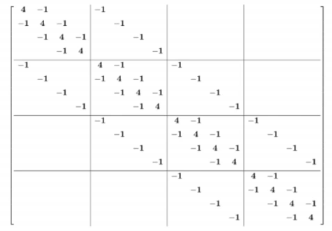
\includegraphics[height=40mm]{matrix.png}
			\caption{Внешний вид матрицы $A$\label{fig:matrix}}
		\end{figure}
		
		Классические прямые методы решения таких систем, например, метод Гаусса или метод матричной прогонки, имеют значительную арифметическую сложность: $O(N^3)$ и $O(N^{2,5})$ соответственно. Это связано с тем, что они не учитывают разреженность блоков матрицы. В связи с этим более эффективными при решении данной задачи оказываются итерационные методы. Так, методы Якоби и Зейделя имеют сложность $O(N^2 \log\frac{1}{\varepsilon})$, а методы ПВР и ADI -- $O(N^{1,5} \log\frac{1}{\varepsilon})$, где $\varepsilon$ - требуемая норма невязки. Тем не менее, это все равно оказывается слишком большой величиной, чтобы применять данные методы на практике: необходимо как можно ближе приблизиться к нижней оценке арифметической сложности, составляющей $O(N)$.
	\section{Метод решения}
		Более эффективным методом для решения данной задачи является метод на основе \textbf{двойного быстрого синус-преобразования}. Его идея состоит в следующем. Имея спектральное разложение матрицы $A=W\cdot D \cdot W^{-1}$, решение системы можно представить в виде $u=W \cdot D^{-1} \cdot W^{-1} \cdot g$. Однако, "в лоб"{} применять этот метод непрактично, так как умножение на $W$ имеет сложность $O(N^2)$. 
		
		Поступим несколько иначе. Собственные числа $A$ и матрица $W$ имеют следующий вид:
		\begin{equation}
		\lambda_{km}=\frac{4}{h^2} \left( \sin\left(\frac{\pi k h}{2}\right)^2 + 
		             \sin\left(\frac{\pi m h}{2}\right)^2 \right)
		\end{equation}
		\begin{equation}
		W_{km,ij} = C\sin(\pi ikh)\sin(\pi jmh),
		\end{equation} где $k$ и $m$ -- горизонтальные и вертикальные индексы узла $p$, т.е. $p=(m-1)(n-1)+k$.
		
		Можно заметить, что умножение на матрицы $W$ и $W^{-1}$ эквивалентно применению прямого и обратного двумерных синус-преобразований, для которых существует алгоритм, аналогичный БПФ и работающий за $O(N\log N)$ операций.
		
		Таким образом, можно предложить следующий метод решения исходной СЛАУ:
		\begin{enumerate}
			\item $v=W^{-1}g$ (обратное 2D ДСП, $O(N\log N)$ операций);
			\item $p=D^{-1}p$ (умножение на диагональную матрицу, $O(N)$ операций);
			\item $u=Wp$ (прямое 2D ДСП, $O(N\log N)$ операций).
		\end{enumerate}
	
		Нетрудно заметить, что предложенный алгоритм имеет сложность $O(N\log N)$, что гораздо ближе к нижней оценке $O(N)$, чем все рассмотренные ранее методы решения СЛАУ.
	\section{Результаты}
		\begin{figure}[h!]
			\begin{minipage}[h]{0.5\linewidth}
				\center{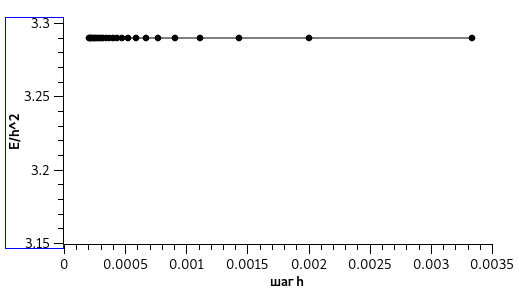
\includegraphics[width=1.0\linewidth]{error.png}}
			\end{minipage}
			\hfill
			\begin{minipage}[h]{0.5\linewidth}
				\center{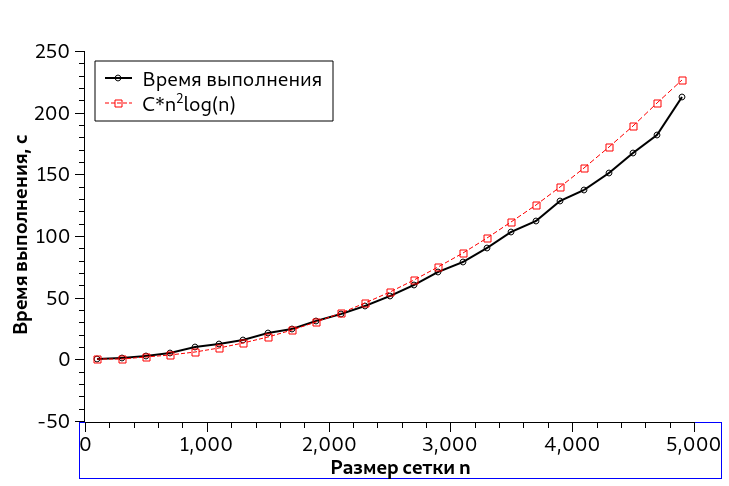
\includegraphics[width=1.0\linewidth]{time.png}}
			\end{minipage}
			\caption{\label{fig:plots} Полученные результаты}
		\end{figure}
		Целью данной работы было реализовать и протестировать рассмотренный выше алгоритм на практике. Полученная программа была написана на языке Python с использованием библиотек SciPy и NumPy. 
		
		Работоспособность программы проверялась на функции $u=\sin(2\pi x)\sin(2\pi y)$, являющейся решением уравнения:
		\begin{equation}
		\Delta u=-8\pi ^2 \sin(2\pi x)\sin(2\pi y)
		\end{equation} 
		
		Тестирование проводилось путем экспериментального вычисления зависимости нормы невязки $E$ и времени работы программы от размерности сетки $n$ (или, что эквивалентно, шага $h$). Результаты представлены на рис.~\ref{fig:plots}. 

	
		Как видно из полученных графиков, предложенный метод правильно решает исходную задачу с порядком аппроксимации $O(h^2)$. Время работы алгоритма совпадает с полученной оценкой $O(n^2\log n)=O(N\log N)$.
	\section{Вывод}
		В данной работе был рассмотрен и успешно реализован на практике метод решения СЛАУ уравнения Пуассона на основе двумерного быстрого синус-преобразования, была показана асимптотическая эффективность данного метода по сравнению с классическими прямыми и итерационными методами решения СЛАУ.
\end{document}